\chapter{Data and methods}
\label{ch:datamethods}
% TODO introduce what is the content of the chapter
\section{Data}
\label{sec:data}
% TODO table overview of the data
% TODO put in each dataset section why you use the data as first paragraph/sentence. SO WHAT??? 
	\subsection{Spatial data}
		\subsubsection{Global Forest Change}
			\ac{GFC} 2000-2012 Version 1.0 is the first high-resolution dataset that provides a comprehensive view of the annual global forest cover change between 2000 and 2012 \citep{Hansen2013, Li2017}. The initial \ac{GFC} dataset released by \citeauthor{Hansen2013} is extended by recent releases which encompass the annual forest cover changes between 2000-2013, 2000-2014, 2000-2015 and 2000-2016, respectively. All versions of this dataset have in common, that they are derived from growing season imagery captured by the remote sensing satellite Landsat 7 \ac{ETM+} enhanced by band metrics of other sensors like Quickbird imagery, existing percent tree cover layers from Landsat data, and global \ac{MODIS} percent tree cover \citep{Hansen2013}. On the satellite imagery, a time-series spectral metrics analysis is applied to gather the global forest extent at 2000 as well as the annual forest loss and the accumulated gain for the period 2001 till 2012. Hence, \ac{GFC} comprises three independent data layers tree cover, annually forest loss and forest gain divided into 10x10 degree tiles by the geodetic coordinate system \ac{WGS84} (EPSG:4326) with a spatial resolution of 1 arc-second per pixel (approximately 900 Km$^2$ or 30x30 m). Furthermore, across the provided \ac{GTiff} layers the pixel data is coded in unsigned 8-bit integers. Hansen et al. defined trees as all vegetation taller than 5 meters for their study. For each pixel covered by trees, a canopy density ranging from 0 t0 100 \% is computed. Forest loss is defined as a stand displacement disturbance leading from a forest state to a non-forest state (e.g. canopy density >50 \% to 0). Tree cover gain is defined as the inverse of loss where the canopy density must exceed 50 \% to get recognized.

			\citeauthor{Hansen2013} reports as an accuracy assessment of tree cover loss a producers accuracy of approximately 83 \% for the tropical region. The mapped tree cover gain is probably an underestimation of the true gain with a producers accuracy of 48 \% and a user's accuracy of 81 \%. 

			This dataset is publicly available for download without any constraint. For a convenient bulk download, the dataset homepage provides a "\verb|*.txt|" files comprising the \ac{URL} of the tiles for each sub-dataset. The spatial location of an image can be directly determined from the file name within the \ac{URL}. Each file name has a common pattern shown by the following expression: "\verb|Hansen_VERSION_LAT[NS]_LNG[WE]|". LAT (latitude) and LNG (logitude) refer to the top left corner coordinates of a raster image, whereas these coordinates are only given in natural numbers. The orientation of the image on the hemisphere is determined by the four cardinal directions N (north), S (south), W (west) and E (east). For this project, we require all three sub-datasets, namely: Treecover2000, lossyear, and gain. The data acquisition is automatized with an Python script by using the \ac{stdlib} modules urllib, re, and threading \citep{Rossum2018}. At first, the Python script downloads the provided "\verb|*.txt|" files and creates a list data structure, where each \ac{URL} is element of this list. After, it cycles through the list and extracts the corner coordinates from the file name by means of a \ac{REGEX}. These corner coordinates and cardinal directions are converted to valid latitude and longitude coordinates between $[-90, 90]$ and $[-180, 180]$, respectively. Now, an image is only downloaded if it is within the study extent between $[-20, 30]$ latitude. The acquired image tiles in total 678 are shown in the top panel (green squares) in figure \ref{fig:tiles}. 
			\begin{figure}[ht]
				\centering
				\includegraphics[scale=.93]{img/tiles}
				\caption[Map of downloaded dataset tiles]{\textbf{Map of downloaded dataset tiles:} This map shows the acquired image tiles for this study. From top to bottom in green Global Forest Change (GFC) dataset tiles (Treecover2000, lossyear and gain), the land cover dataset GlobeLand30 (GL30) image tiles in red, and in blue the Aboveground Biomass (AGB) dataset tiles. The orange filled shapes highlight countries within the tropical zone.}
				\label{fig:tiles}
			\end{figure}

		\subsubsection{GlobeLand30}
			\ac{GL30} is the first global land cover dataset with a 30 meter per pixel spatial resolution that provides a comprehensive view on the distribution of 10 different land cover classes (table \ref{tab:gl30classes}) over the entire globe \citep{Chen2017}. Currently this dataset is available for two different time periods 2000 and 2010 \citep{Chen2015}. The pixel values of this dataset are coded in unsigned 8 bit integers and as coordinates system it uses \ac{WGS84} in \ac{UTM} projection. \ac{GL30} can be downloaded as a \ac{GTiff} raster mosaic where each image covers 6x5 degrees \citep{Chen2014}. For detecting the land cover classes \citeauthor{Chen2015} used a so called \ac{POK} oriented approach and satellite imagery from Landsat \ac{ETM+} \citep{Chen2015}. \citeauthor{Chen2015} divided the mapping process in different stages where each land cover type is detected separately and deleted subsequently from the source satellite image. The applied mapping order is: water bodies, wetland, snow and ice, cultivated land and forest, shrubland, grassland and bareland synchronous. To detect the pixels of a selected land cover type the following pixel level classifiers are used: \ac{DT}, \ac{SVM} or \ac{MLC}. After pixel detection the adjacent pixels are grouped as an aggregated land use object. These objects are subsequently validated by expert knowledge and the gained knowledge is used as a feedback loop to improve the automatized classification.

			\citeauthor{Chen2015} estimates an overall mapping accuracy of 80.33 \% and 78.6 \% for 2000 (only validated in Shaanxi, China) and 2010 (global), respectively \citep{Chen2015}. Several research groups besides \citeauthor{Chen2015} validated the mapping accuracy of \ac{GL30} at different regions and scales. \citeauthor{Arsanjani2016} estimates an overall accuracy of 77.9 \% for Iran and an accuracy >80 \% for Germany \citep{Arsanjani2016a,Arsanjani2016}. Yang et al., Cao et al. and Jacobson et al. estimate an accuracy of 82.4 \%, 80.1 \% and 83.1 \% for China, Nepal and East Africa, respectively \citep{Yang2017,Cao2016,Jacobson2015}. Unfortunately, no study focused on validating the mapping accuracy for regions exclusively within the tropical zone.

			\citeauthor{Chen2015} donated the \ac{GL30} land cover mapping to the \ac{UN} but it is not accessible for public download. The download is restricted to users who register on the dataset homepage but the registration process is not working properly. Fortunately the supervisor of this work had already an account otherwise it would be impossible to receive a copy of the dataset. A registered user must fill an order application to get access to the image tiles. The application form must contain the tile identifiers and the selected time period. Tile identifiers have the following common pattern: "\verb|[NS]ZONE_LAT_NAME|" where zone refers to the \ac{UTM} zone between $[1, 60]$, N (north) or S (south) to the cardinal direction, and LAT (latitude) to the latitude coordinate of the top left corner. For a better usability the homepage provides an interface for selecting the required image tiles but the selection of multiple tiles did not work. As well a vector file is provided which contains the dataset tile polygons with assigned identifiers. This file was used to select all required tiles within the tropical zone between approximately $[-23, 23]$ degrees (\ac{WGS84}). Figure \ref{fig:tiles} presents the selected images in red at middle panel. The corresponding image identifiers are converted to an single line string and copied to the application form. After submitting the form the order will be checked and approved within two weeks. After one week we received a two weeks limited access to an password protected \ac{FTP} server where we downloaded 716 raster images. Due to the several restrictions this process of selecting and downloading could not be automatized with one pipeline. Only the selection and string conversion was automatized with a throw away script.
			\begin{table}[ht]
				\centering
				\caption[Classification schema of the GlobeLand30 product]{\textbf{Classification schema of the GlobeLand30 product:} The code column is the assigned pixel value, type the corresponding land cover type and definition explains in broad terms which types of surfaces fall into the land cover type \citep{Chen2017}.}
				\label{tab:gl30classes}
				\begin{tabular}{rlp{10.3cm}}
					\hline
					Code & Type & Definition \\\hline
					10 & Cultivated land & used for agriculture, horticulture and gardens, including paddy fields, irrigated and dry farmland, vegetable and fruit gardens, etc. \\
					20 & Forest & covered by trees, vegetation covers over 30 \%, including deciduous and coniferous forest, and sparse woodland with cover 10-30 \%, etc. \\
					30 & Grassland & covered by natural grass with cover over 10 \%, etc.\\
					40 & Shrubland & covered by shrubs with cover over 30 \%, including deciduous and evergreen shrubs, and desert steppe with cover over 10 \%, etc.\\
					50 & Wetland & covered by wetland plants and water bodies, including inland marsh, lake marsh, river floodplain wetland, forest/shrub wetland, peat bogs, mangrove and salt marsh, etc.\\
					60 & Water bodies & in land area, including river, lake, reservoir, fish pond, etc.\\
					70 & Tundra & covered by lichen, moss, hardy perennial herb and shrubs in the polar regions, including shrub-, herbaceous-, wet- and barren-tundra, etc.\\
					80 & Artificial surfaces & modified by anthropogenic influence, including all kinds of habitation, industrial and mining area, transportation facilities, and interior urban green zones and water bodies, etc.\\
					90 & Bareland & with vegetation cover lower 10 \%, including desert, sandy fields, Gobi, bare rocks, saline and alkaline land, etc.\\
					100 & Snow and ice & covered by permanent snow, glacier and icecap\\\hline
				\end{tabular}
		\end{table}

		\subsubsection{Intact Forest Landscapes}
			A \ac{IFL} is a mosaic of undisturbed forest patches and naturally treeless ecosystems without sings of human activity and large enough to maintain all native biological diversity \citep{Potapov2017}. Due to the fact that \ac{IFL} comprises different intact natural landscape patterns like primary forests, non-forest ecosystems, temporary treeless areas after a natural disturbance, and water bodies the term is not congruent to the term primary forest defined by the \ac{FAO} \citep{FAO2012}. But as mentioned \ac{IFL}s includes large patches of primary forests with a minimum extent of 500 Km$^2$ therefore primary forests can be extracted from the layer. Still there are smaller fragments of primary forest outside of the \ac{IFL}s. In regards of the extent an \ac{IFL} has a minimum size of 500 Km$^2$, a minimum width of 10 Km, and a minimum corridor/appendage width of 2 Km. Further an \ac{IFL} should not contain any of the following: ecosystem alternation, fragmentation by infrastructure and disturbance, and areas altered or managed trough agriculture, logging, and mining. For mapping and detecting \ac{IFL}s \citeauthor{Potapov2017} used Landsat imagery and several auxiliary data sources like \ac{GFC}, and national transportation maps. The dataset can be downloaded as a \ac{SHP} file with the coordinate reference system \ac{WGS84}. Each polygon in the \ac{SHP} represents an \ac{IFL} patch at a certain location on our planet at the time period 2000.

			Data acquisition is pretty straight forward the \ac{IFL} dataset public accessible for download. As mentioned it is an \ac{SHP} so you must only download a single compressed archive. The download is automatized with an Python script by using the \ac{stdlib} modules urllib and threading \citep{Rossum2018}.

		\subsubsection{Aboveground Woody Biomass}
			The \ac{AGB} raster dataset is prepared by \ac{GFW} by an adapted approach of \citeauthor{Baccini2012} \citep{Baccini2012,Baccini2015,Baccini2017}. For the year 2000, this dataset estimates the aboveground biomass density per pixel in Mg C ha$^{-1}$ (mega gram carbon per hectare), and the confidence per pixel at a spatial resolution of approximately 1 arc-second (approximately 900 Km$^2$ or 30x30 meter). The dataset covering the global tropical zone as an mosaic of \ac{GTiff} raster images where each tile of the mosaic has the \ac{CRS} \ac{WGS84} and is coded in float. For deriving biomass density \ac{GFW} used canopy metrics from \ac{GLAS} \ac{LIDAR} footprints and several regional and forest specific allometric equations. The resulting \ac{GLAS} \ac{AGB} estimates are used as labels to train regional specific \ac{RF} models based on Landsat 7 \ac{ETM+} top-of-atmosphere reflectance, tree canopy density of \ac{GFC}, elevation data, and climate data as predictor variables. After these models are subsequently applied to the entire study extent to predict the biomass content for each pixel. Additional a uncertainty layer is prepared accounting for the errors from allometric equations, the \ac{LIDAR} based model, and the random forest model.

			The \ac{AGB} raster mosaic is public available on the homepage of \ac{GFW}. As mentioned, the dataset covers only the tropical zone, therefore we acquires the entire mosaic. The \ac{GFW} homepage provides an \ac{GeoJSON} \ac{API} to receive the actual \ac{URL} of each raster image. If a request is send to this \ac{API} the server response with a \ac{GeoJSON} feature collection. The collection contains as attributes the \ac{URL}s of the biomass images, the \ac{URL} of the uncertainty layers, and the rectangular bounds of each image. The data acquisition is automatized by means of Python and the \ac{stdlib} modules urllib, threading, and the open source library geopandas \citep{Rossum2018,McKinney2010}. At first the \ac{GeoJSON} is downloaded via an \ac{API} call and eventually stored on disk. Next we iterate the features of the \ac{GeoJSON} collection and extract the \ac{URL}s (biomass and uncertainty) of each tile. These \ac{URL}s are downloaded and subsequently stored on disk. During the downloads of the uncertainty layers the \ac{GFW} server answered repeatedly with a 404 (Not found). Therefore the uncertainty layers are not available. In total we downloaded 105 different image tiles, their extent and spatial location is shown in blue at the bottom panel of figure \ref{fig:tiles}.

		\subsubsection{Global Soil Organic Carbon}
			% TODO references for wosis, hwsd, and other data products
			The \ac{GSOCmap} is a joint project between \ac{GSP} and \ac{ITPS} to produce a global \ac{SOC} content map by a country driven approach. In the year 2018, the first iteration of this map in version 1.0 was released, and shortly followed by 1.1 (new country submission by Rwanda) and 1.2 (new country submissions by Chile and Colombia). As the short release cycle suggests the mapping project is intended as a long-lived dataset which will improve over time and by new country submissions. Till now 67 (approximately 63 \% of the global land mass) different countries submitted their country based \ac{SOC} estimates. To foster the national \ac{SOC} mappings the \ac{ISRIC} provides several covariate datasets like national \ac{DEM} maps, annual spectral remote sensing data or national soil type grids. Additionally the contributors can join a mapping training and use the \ac{GSOCmap} cookbook as guidance for their mapping efforts. As an exchange, each country shares its national \ac{GSOCmap} by compliance of several criteria e.g. reporting of the Meta-data of the \ac{SOC} sampling (sample timeline, sample depth, bulk density etc.), uncertainty assessment, and the applied methods for estimating and interpolation of the \ac{SOC} content. For interpolating the guide organizations suggest the following approaches: simple geo-matching, class-matching, \ac{MLR}, \ac{RF} or \ac{SVM}. The national maps are aggregated to the final \ac{GSOCmap} with a target resolution of 30 arc-seconds (approximately 1 Km$^2$) in the \ac{CRS} \ac{WGS84}. The dataset is one single raster image as \ac{GTiff} coded in float covering the entire globe where each pixel value is the \ac{SOC} content in Mg C ha$^{-1}$ at a soil depth of 0-30 cm \citep{FAO2018}.

			The product is validated by comparing the pixel level estimates with soil sampling data from various soil databases (WoSIS, HWSD, etc.). In total 312122 samples where divided into three sub-levels (<150 Mg C ha$^{-1}$, >150 Mg C ha$^{-1}$, and all samples) and subsequently computed the \ac{ME}. The \ac{ME} of the entire sample space and <150 Mg C ha$^{-1}$ suggests that the mean \ac{SOCC} estimate is an overestimate of 1.6 and 4.5 Mg C ha$^{-1}$ respectively. All samples with a \ac{SOCC} content >150 Mg C ha$^{-1}$ show an underestimate by approximately 165 Mg C ha$^{-1}$ in the mean. Additionally, an uncertainty assessment was prepared to estimate a \ac{SD} between $\pm$ 0-16 t ha$^{-1}$ for the tropical zone. Unfortunately, is this assessment pretty rough and till now not available as a product. The \ac{GSOCmap} in comparison with other global \ac{SOC} products has the lowest \ac{RMSE}. In summary, the prepared validations show evidence that the \ac{GSOCmap} is a conservative data product with a tendency to underestimate the \ac{SOCC}.

			The dataset is publicly available at the homepage of the \ac{FAO}. As mentioned it consists of one raster image, therefore we download it by means of a Python script without any additional steps.

		\subsubsection{Auxiliary}
			As auxiliary data for country boundaries we downloaded with Python the \ac{GADM} layers as \ac{SHP} files \citep{Hijmans2018,Rossum2018}.

	\subsection{Empirical data}
		\subsubsection{Soil Organic Carbon}
			\citeauthor{Don2010} performed the first study of tropical \ac{SOC} change for soil depth between 0 and 30 cm. For the study a global meta-analysis is applied by using 358 (153 published an peer-reviewed) different studies to estimate \ac{SOC} change for 12 major \ac{LUC} types. The base date is derived from 39 different tropical countries covering all continents. Unfortunately Africa and East-Asia are under-sampled whereas South-America have the best data coverage. The meta-analysis is restricted to mineral soils therefore all wet soil types are excluded from the analysis \citeauthor{Don2010}. The 12 \ac{LC} transitions encompass the following \ac{LC} types: primary forest, secondary forest, grassland, cropland, and perennial crops. Primary forest are defined as natural vegetation without human impacts which includes natural grassland and shrubland. Secondary forest are managed forests and regrown forests after partial destruction of the old stand. Grassland comprises pastures for livestock but excludes natural grasslands. Cropland comprises annual crops like maize or beans and perennial crops could be coffee or sugar cane. For our study we used only the \ac{SOC} change estimates for these \ac{LUC} types which corresponds to the \ac{GL30} and \ac{IFL} classification schema. The actual values are shown in table \ref{tab:soc}.
			\begin{table}[ht]
				\centering
				\caption[Relative soil organic carbon change for certain land-use change types]{\textbf{Relative soil organic carbon change for certain land-use change types:} The Land-use change columns from and to define the LUC type with the corresponding relative Soil Organic Carbon (SOC) change and the Standard Error of the Mean (SEM) \citep{Don2010}.}
				\label{tab:soc}
				\begin{tabular}{ccrr}
					\hline
					\multicolumn{2}{c}{LUC type} & \multicolumn{2}{c}{Relative SOC change} \\
					From & To & [\%] & SEM \\\hline
					Primary forest & Grassland & -12.1 & $\pm$2.3 \\
					Primary forest & Cropland & -25.2 & $\pm$3.3 \\
					Primary forest & Secondary forest & -8.6 & $\pm$2.0 \\
					Secondary forest & Grassland & -6.4 & $\pm$2.5 \\
					Secondary forest & Cropland & -21.3 & $\pm$4.1 \\\hline
				\end{tabular}
			\end{table}

		\subsubsection{Ecosystem Service Values}
		% TODO write the section, improve caption
			Some text to ensure document flow.
			\begin{table}[ht]
				\centering
				\caption[Selection of Ecosystem Service Values (ESV) used in this study]{\textbf{Selection of Ecosystem Service Values (ESV) per biome used in this study:} ESV per biome connected with the corresponding GlobeLand30 land-cover class, and its monetary value in Int.\$ ha$^-1$. Dg refers to data from \citeauthor{Groot2012}, Co from \citeauthor{Costanza2014}, and Wb from \citeauthor{Siikamaki2015}.\citep{Groot2012,Costanza2014,Siikamaki2015}}
				\label{tab:esv}
				\begin{tabular}{lclrrr}
					\hline
					Biome & Code & Type & Dg & Co & Wb \\\hline
					Cropland & 10 & Cropland & - & 5,567 & -\\
					Forest tropical & 20 & Forest & 5,264 & 5,382 & 1,312\\
					Forest tropical & 25 & Regrowth & 5,264 & 5,382 & 1,312\\
					Grass/Rangelands & 30 & Grassland & 2,871 & 4166 & -\\
					Wetlands & 50 & Wetland & 25,682 & 140,174 & -\\
					Lakes/Rivers & 60 & Water bodies & 4,267 & 12,512 & -\\
					Urban & 80 & Artificial & - & 6,661 & -\\\hline
				\end{tabular}
			\end{table}

\section{Methods}
\label{sec:methods}
%TODO need more speacking section headings
% TODO put in each dataset section why you use the data as first paragraph/sentence. SO WHAT???
	\subsection{Preprocessing}
		%TODO improve flowchart final masking, improve caption
		Before we apply further analysis, we have to generalize the used datasets. As introduced in the data section do we use datasets which differ largely in their metadata properties, for example, single-tiled or multi-tiled images, used \ac{CRS}, spatial resolution, and file type. Therefore, our goal should be to develop a process which creates an image stack of equal meta-data for each location in our study extent. In further descriptions, we will refer to this stack as \ac{AISM}. As target \ac{CRS} for our \ac{AISM} we chose \ac{WGS84} and as target extent for the mosaic, we use the bounding box of the \ac{GL30}-2010 tiles. The following paragraph explains how we developed the alignment algorithm by means of Python and the additional open source libraries rasterio, geopandas, and shapely \citep{Rossum2018,McKinney2010}.

		The first exercise of the preprocessing algorithm is to detect all tiles covering the extent of our template tiles. At first, we create for each multi-tiled dataset a polygon mask as \ac{SHP}. This mask contains the spatial extent of each tile within a dataset and as attribute the corresponding file identifier. If the dataset tiles are not in \ac{WGS84} the extracted bounds are subsequently reprojected to this \ac{CRS}. During the masking process, we recognized that the raster mosaic bounds of both \ac{GL30} datasets (2000 and 2010) generate re-projection errors. These errors showed up as polygons spanning the entire globe but one tile can only fill its \ac{UTM} zone extent. A further analysis revealed that all tiles located in \ac{UTM} zone 1 and 60 overflowing the maximum and minimum longitude coordinates of this zones. As solution we excluded all tiles within \ac{UTM} zone 1 and 60 from further processing, namely: n01\_00, s01\_00, s01\_10, s01\_15, s01\_20, s60\_00, s60\_05, s60\_10, s60\_15, and n53\_00. The described steps can be found as well in figure \ref{fig:preprocessing_flowchart}. Now, as the figure suggests we determine the intersection between these mask layers and group the intersecting tiles by our template tile. Next, we create for the template tile a re-projection profile (warp profile) and apply it subsequently to all intersecting tiles based on the following rules: if from one dataset more than one tile intersects merge them followed by re-projection or if only one tile intersects just re-project it. As introduced the \ac{GSOCmap} consist only of one single tile with a spatial resolution of approximately 1 Km$^2$, so it must only re-project and re-sampled by nearest-neighbor approach. We select from the \ac{IFL} layer all polygons within our template warp profile and convert them to a raster layer where intact forest patches are coded by a one in 8-bit unsigned integer. Last step of the alignment process is the rounding of the \ac{AISM} bounds to full integer degrees and a subsequent clipping of each tile to this rounded bounds. The entire work flow it pictured in figure \ref{fig:preprocessing_flowchart} and results in a \ac{AISM} shown in figure \ref{fig:aism}. Finally, we create a polygon mask of our \ac{AISM} and store for each polygon the corresponding dataset tiles. This mask is used as a file index for the next algorithms.
		\begin{figure}[ht]
			\centering
			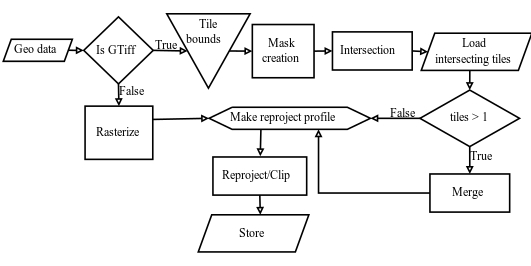
\includegraphics[scale=.8]{img/align}
			\caption[Flowchart of tile alignment process]{\textbf{Flowchart of tile alignment process:} For the multi-tiled datasets (multi-document symbols) a mask is created by extracting the tile bounds. Next, the intersection between theses masks is determined and the corresponding tiles are loaded from disk. \ac{GL30} tiles are used as template by creating re-project profile and subsequently applying it to intersecting tiles. From the \ac{IFL} layer only polygons within the re-project are selected and subsequently converted to a raster layer.}
			\label{fig:preprocessing_flowchart}
		\end{figure}
		\begin{figure}[ht]
			\centering
			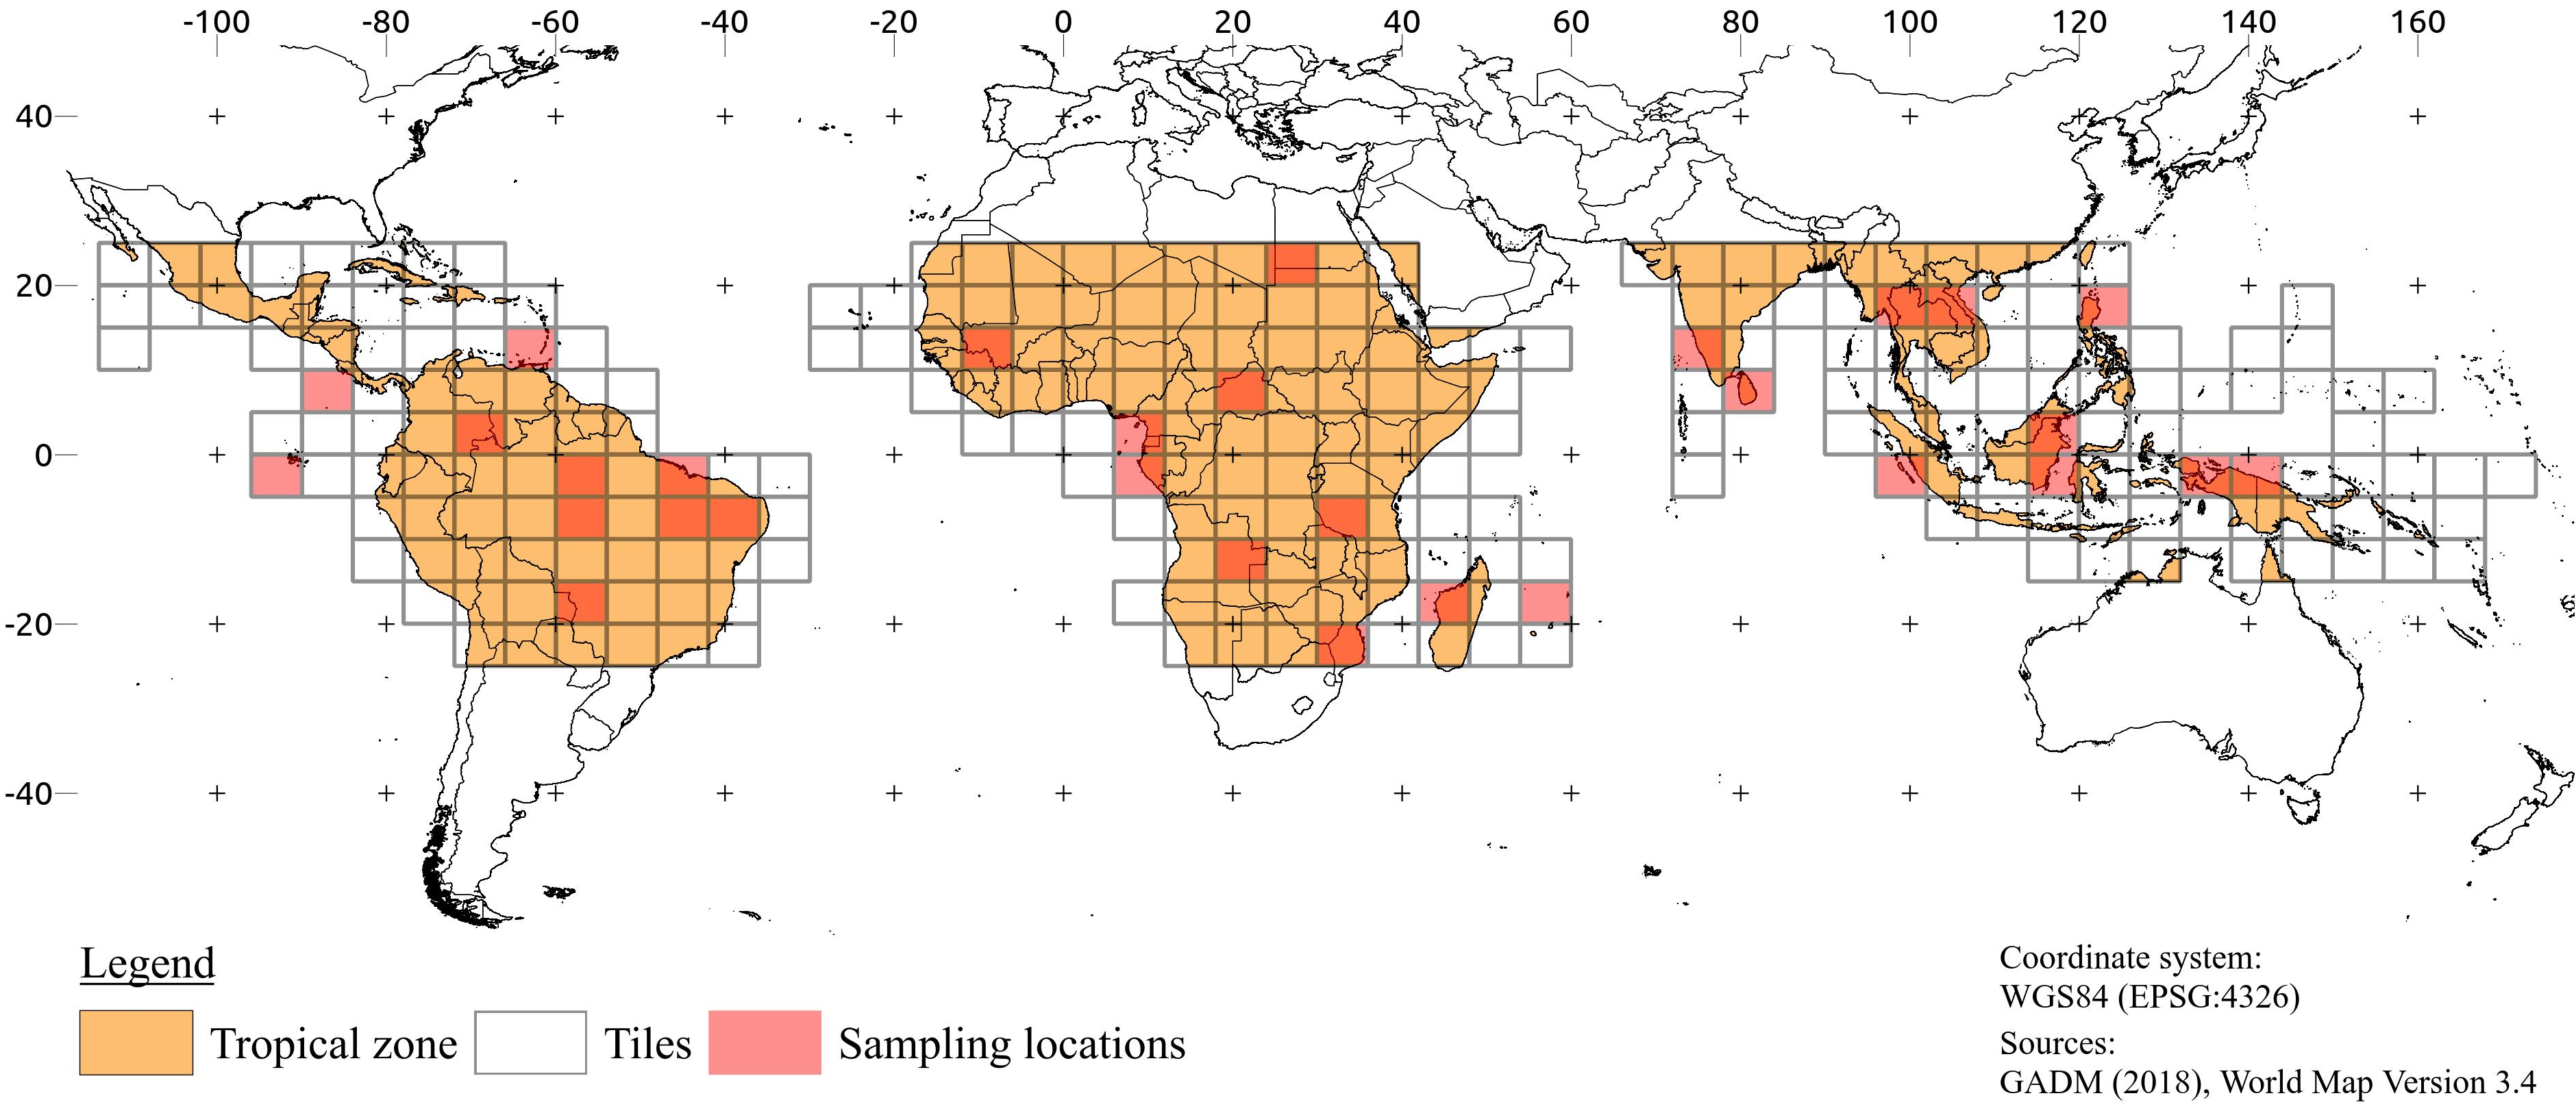
\includegraphics[scale=.91]{img/method_overview_frameless}
			\caption[Map of aligned data tiles and sampling locations]{\textbf{Map of aligned data tiles and sampling locations:} The map shows the location of the aligned multi-image stack tiles as black-framed square sized polygons, the sampling locations for accuracy assessment in red, and countries within the tropical zone in orange.}
			\label{fig:aism}
		\end{figure}

	\subsection{Deforestation}
		\subsubsection{Forest definition}
			Treecover agreement: Jaccard index first applied for a study on plant distribution similarities at different locations in alps and developend by jaccard \citep{Jaccard1912,Shi1993,Sampat2009} jaccard index, wilcoxon signed-rank test, gl30 2000, gfc treecover 2000, different canopy densities JI$_0$$[0,100]$, JI$_{1}$$(10,100]$, JI$_{2}$$(20,100]$, JI$_{3}$$(30,100]$ 

		\subsubsection{Proximate deforestation driver}
			%TODO flowchart needs reclassification
			Based on our forest definition developed in the previous section we want to classify all the tropical deforestation within a canopy density of $(10,100]$ percent between 2001 till 2010. Additionally we must consider the mean miss-classification rate of 52 \% by previous findings of \citeauthor{Seydewitz2017} \citep{Seydewitz2017}. Therefore we have to develop a feasible method to resolve this issue.

			For classifying the proximate drivers of deforestation we select the following raster images from our \ac{AISM}: \ac{GFC} treecover2000, \ac{GFC} lossyear, \ac{GFC} gain, and the \ac{GL30} \ac{LC} classification from 2010. Now, we apply to each raster image stack the following described operations. From the treecover2000 layer we select all pixels where the canopy density is within $(10,100]$ percent and set them to one (true). The same is procedure is applied on the lossyear layer by setting all forest loss pixels within the time period 2001 till 2010 to one (true). After both layers are combined with a logical AND to select our target deforestation pixels. Finally, we build the Hadamard product (element-wise multiplication) of the target deforestation layer and the \ac{GL30} \ac{LC} layer to classify the deforestation pixels. Last step is to add the forest gain layer 
			use the hadamard product to classify the target deforestations with the \ac{GL30} layer. For classifying the regrowth 
			The classification is implemented as a Python function which requires as parameter the previously named raster layers. Additionally the target canopy density and time period is freely selectable.

			Classification: We from our AISM treecover 2000, lossyear, gain and gl30 2010. select from all pixels within 11 and 100 canopy density and set them to 1, from lossyear losses between 2001 and 2010, additionally  we filter losses so they are only in our target canopy density and set them to 1, now do the hadamard product with the gl30 layer, last step is to filter gain within our loss layer and to add it to the hadamard product as 25, this is regrowth.

			Resolve classification issues: 
			\begin{figure}[ht]
				\centering
				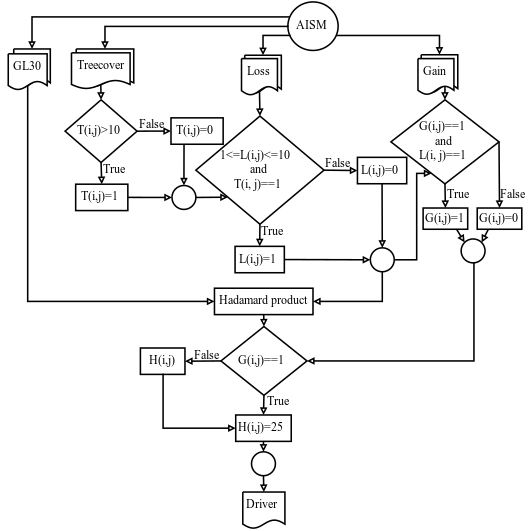
\includegraphics[scale=0.5]{img/driver_flowchart}
				\caption[]{\textbf{Title:}}
				\label{fig:driver_flowchart}
			\end{figure}

		\subsubsection{Accuracy assessment}
			For examining the accuracy of our proximate deforestation driver prediction we used a confusion matrix (also known as two-way frequency tables, error matrix or contingency tables). These matrices are commonly used for an accuracy assessment of land cover classifications and enables the computation of marginal and conditional distributions \citep{Congalton1991,Foody2002}. Table \ref{tab:confusion} shows a general model of a confusion matrix. Foundation for an accuracy assessment by means of a confusion matrix is a collection of ground-truth samples which can be compared with the class predictions for these samples produced by a classification algorithm. For the preparation of our accuracy assessment, we have to extract a collection of pixel samples with a deforestation occurrence from our proximate  driver maps (further also called predictions). Next, we compose a set of ground-truth for these predictions (further also called references).
			\begin{table}[ht]
				\centering
				\caption[A general model of a confusion matrix]{\textbf{A general model of a confusion matrix:} $X_1$, ... , $X_n$ denote classification categories of two independent raters. $x_{n,n}$ are the actual samples sorted into the categories where the values in the diagonal show the agreement between both raters. The remaining cell values account for the disagreement between the two raters. $\sum$ column and row show the marginal distribution and N is the total number of samples.}
				\label{tab:confusion}
				\begin{tabular}{lccccc}
					\hline
					& & \multicolumn{3}{c}{Reference} & \\
					& Cls & $X_1$ & $\cdots$ & $X_n$ & $\sum$ \\\hline
					\multirow{4}{*}{\STAB{\rotatebox[origin=c]{90}{Predict}}}
					& $X_1$ & $x_{1,1}$ & $\cdots$ & $x_{1,n}$ & $x_{1.}=
					\displaystyle\sum_{i=1}^{n} x_{1,i}$ \\ 
					& $\vdots$ & $\vdots$ & $\ddots$ & $\vdots$ & $\vdots$ \\ 
					& $X_n$ & $x_{n,1}$ & $\cdots$ & $x_{n,n}$ & $x_{n.}=\displaystyle\sum_{i=1}^{n}x_{n,i}$ \\\hline 
					& $\sum$ & $x_{.1}=\displaystyle\sum_{i=1}^{n}x_{i,1}$ & $\cdots$ & $x_{.n}=\displaystyle\sum_{i=1}^{n}x_{i,n}$ & $\sum\sum=N$ \\\hline
				\end{tabular}
			\end{table}

			To create our collection of ground-truth data we draw randomly 10 image tiles from all three continental regions (Latin America, Africa, Asia/Oceania). From each tile, we sampled by random 200 pixels which total to 6000 samples over the entire study region. The sampling is realized with our own raster sampling algorithm build in Python by means of the open source libraries numpy and rasterio. As mentioned in the previous section do we superimpose two datasets and only a certain amount of pixels per tile is classified as proximate driver. Therefore, the sampling algorithm should only draw samples from occupied/classified pixels without replacement. The algorithm expects as parameters a raster image, the total number of samples to draw, a list of pixel values which should be interpreted as occupied cells, the affine transformation matrix of the raster image, and a seed for the random number generator. If occupied cells are set the algorithm will create a binary mask where each occupied cell is set to one relative to the input raster image. Otherwise it sets all pixel values greater or less than zero to one. After, the row and column coordinates of each one are extracted from the mask and converted to a flat list of coordinate tuples. Next, it draws the predefined number of samples from the list by a random order and uses the image coordinates to get the pixel value from the raster image. If a affine transformation matrix is provided the image coordinates are converted to real world coordinates. The seed argument ensures that on every algorithm rerun the samples are drawn. For our sampling we set the parameters to the following values: samples 200, occupied pixels \ac{GL30} class values and 25 for regrowth, affine matrix of the corresponding raster image, and the seed is 42. The per tile samples are stored as an \ac{CSV} file.

			For the collection of ground-truth data we used visual interpretation of Google Earth satellite and aerial imagery. We developed a small JavaScript web application to access the imagery via the Google Maps \ac{API}. The application expects as input a \ac{CSV} file with the sampling coordinates. After upload of a sample file the user can cycle trough the entries and the map jumps automatically to the coordinates of the sample. Now a reference label can be assigned to the coordinates by visual interpretation of the imagery. We subsequently assigned to all 6000 samples a reference label and downloaded the results as \ac{CSV}.

			Finally, we developed a Python class to compute the confusion matrix. The constructor of the class requires a list of reference and prediction labels. With the provided arguments it creates the confusion matrix. Further, it computes the following marginal and conditional distributions: overall accuracy $OvAc$ by dividing the sum of classification agreements trough the sample total $N$ (equation \ref{eq:OvAc}), the producer accuracy $PAc_{.n}$ by dividing the category agreement trough the column category total (equation \ref{eq:PAc}), the error of commission $Com_{.n}$ (Type II error) by dividing the category disagreement trough the column category total (equation \ref{eq:Com}), the user accuracy $UAc_{n.}$ by dividing the category agreement trough the row category total (equation \ref{eq:UAc}), the error of omission $Om_{.n}$ (Type I error) by dividing the category disagreement trough the row category total (equation \ref{eq:Om}), and the Cohens Kappa by substituting equation \ref{eq:cohen} and \ref{eq:OvAc} into equation \ref{eq:Kappa}.
			\begin{equation}
			\label{eq:OvAc}
				p_0=OvAc = \frac{\displaystyle\sum_{i=1}^{n}x_{i,i}}{N}
			\end{equation}
			\begin{equation}
			\label{eq:PAc}
				PAc_{.n} = \frac{x_{i,i}}{x_{.n}}
			\end{equation}
			\begin{equation}
			\label{eq:Com}
				Com_{.n} = \frac{FN_i}{x_{.n}}
			\end{equation}
			\begin{equation}
			\label{eq:UAc}
				UAc_{n.} = \frac{x_{i,i}}{x_{n.}}
			\end{equation}
			\begin{equation}
			\label{eq:Om}
				Om_{n.} = \frac{FP_i}{x_{n.}}
			\end{equation}
			\begin{equation}
			\label{eq:cohen}
				p_c = \frac{1}{N^2}\displaystyle\sum_{i=1}^{n} x_{.i} \cdot x_{i.}
			\end{equation}
			\begin{equation}
			\label{eq:Kappa}
				Kappa = \frac{p_0-p_c}{1-p_c}
			\end{equation}

	\subsection{Emissions}
		\subsubsection{Above ground biomass}
			\lipsum[1-2]
		\subsubsection{Soil organic carbon change}
			\lipsum[1-2]

	\subsection{Ecosystem service values}
		\subsubsection{Ecosystem service value loss}
			\lipsum[1-2]
		\subsubsection{Ecosystem service value gain}
			\lipsum[1]

	\subsection{Binning analysis}
		% TODO REVIEW, CHANGE TO GOOD ENGLISH
		The previous sections were focused on the generation of large scale spatial data. Now, a feasible method must be developed for analyzing, aggregating, interpreting, and visualizing our results. For the development of a proper approach we have to generalize the problem domain. At first we are confronted with large N (many samples) which results in a high dimensionality and complexity of relationships among this variables \citep{Carr1990}. From a visual/analytical perspective georeferenced raster maps can be interpreted as a multivariate scatter plot of large datasets where longitude and latitude represent the x and y coordinate of an data point and the pixel values (in this case nominal scaled) representing the third dimension as an group coloring. Therefore we have a large multidimensional dataset combined with a scatter plot visualization which leads commonly to over plotting issues and hidden point densities \citep{Carr1987}. Due to the spatial nature of your data we are also confronted with not equal distributed data some regions show high data densities and other regions have sparse to no data. Also a severe problem domain is the frame size of our representation. Goal is to present data on a continental level which intensifies visual problems. Each pixel has a resolution of approximately 30x30m, the continental representation of americas spanning approximately 1200000x120000km2. Therefore small scale isolated changes are hidden and only large scale changes are visual detectable. Which results in hidden details and not perceivable patterns of change.

		% TODO REFERENCE FOR MAJOR RESAMPLING APPROACH
		% TODO DESCRIBE ADVANTAGES DISADVANTAGES OF VARIOUS TESSELATIONS
		Goal should be to develop an process who solve this issues and generates satisfying output for our multivariate data. In case of raster data a re-sampling to coarser resolution could solve over plotting and resolution issues as well normalize the unequal distributed data. But the nature of re-sampling (for nominal data a nearest neighbor or majority wins \note{Reference}) would negate important spatial patterns as well frequency distributions. Another well known approach is to use binning of the spatial explicit data with a certain kind of regular polygon that is tessellating the plane \citep{Carr1992}. Polygon tessellations provide numerous opportunities for presenting multivariate statistical summaries. The scaling of the polygon could be used to represent pixel densities within the polygon area, a polygon filling color gradient is applicable to show nominal or ordinal scaled data. Also it is imaginable to use the polygon interior for a pie chart. To use regular tessellation it is important to mention there are only three types of regular polygons tessellate the plane: squares, equilateral triangles and hexagons \citep{Carr1992}. Square tessellation is the most common approach used for binning in spatial visualization. A raster image is a square tessellation. In a square mosaic each polygon shares 4 edge neighbors and 4 vertex neighbors \note{more explanation error distance disadvantages etc Hexagons properties, advantages disadvantages of both tessellations}. Final goal is to show your analysis results of spatial explicit raster data in hexagonal binned form. For bivariate maps we choose a visual representation with scaled hexagons and colorization. For multivariate details we choose a pie chart alike visualization. We split the hexagons horizontal in regards of the presented ratio. The ratios should be ordered descending so that the greatest ratio is south oriented. It is following a general description how we created the hexagon grids and how we tackled the polygon split problem. 

		% TODO REFERENCE IMAGE BETTER
		To be flexible at hexagon construction we accept 4 different parameters as construction arguments: $D$ long diagonal (Diameter of the circumscribing circle), $d$ short diagonal (diameter of the inscribed circle), $A$ area the hexagon should span and or $e$ the edge length. One selected parameter of these is used to compute $R$ the radius of the circumscribing circle with respect to input parameter as shown in  equation \ref{eq:paramters}. R is used to calculate the midpoint $<c_x, c_y>$ of the hexagon located in the first quadrant of the cartesian coordinate system Equation \ref{eq:centerx} and \ref{eq:centery}. Equation \ref{eq:hexagon} shows the computation of the hexagon anti-clockwise vertex matrix. Whereas the two leftmost vertices (first and last row of the matrix $\textbf{H}$) are located at koordinatenursprung, will sagen auf deutsch korridanten at x=0 und y=value of matrix. In summary equation \ref{eq:paramters} to \ref{eq:hexagon} show the creation of an hexagon at the leftmost corner of first quadrant (Figure \ref{fig:hexagon}). The orientation is important for the subsequent mosaic creation.
		\begin{equation}
		\label{eq:paramters}
			R = \frac{\sqrt{2A}}{\sqrt[4]{27}} = \frac{D}{2} = \frac{d}{\sqrt{3}} = e
		\end{equation}
		\begin{equation}
		\label{eq:centerx}
			c_x = \frac{R\sqrt{3}}{2} 
		\end{equation}
		\begin{equation}
		\label{eq:centery}
			c_y = R
		\end{equation}
		\begin{equation}
		\label{eq:hexagon}
			\mathbf{H} =
			\begin{bmatrix}
				0 & c_x & 2c_x & 2c_x & c_x & 0 \\
				R\sin\left(\frac{7\pi}{6}\right) + c_y & 0 & R\sin\left(\frac{11\pi}{6}\right)+c_y & R\sin\left(\frac{\pi}{6}\right)+c_y & 2R & R\sin\left(\frac{5\pi}{6}\right)+c_y \\
				1 & 1 & 1 & 1 & 1 & 1
			\end{bmatrix}
		\end{equation}
		% TODO BENCHMARK FUNCTIONS
		% TODO FINISH TESSELATION DESCRIPTION USE IMAGE
		A polygon tessellation needs several polygons to create a grid in case of the creation of one hexagon with the presented algorithm needs approximately \note{benchmark} but the creation of \note{several N hexagons} needs approximately \note{benchmark}. Therefore it is much simpler to create only one hexagon with the presented algorithm and to create the grid polygons by copying the coordinates of the source polygon and translating them to their target position with a affine transformation matrix shown in equation \ref{eq:translate}. To create the grid we get the rectangular bounds of the area to tessellate as a matrix $\textbf{B} \in R^{2\times2}$ (equation \ref{eq:bounds}), where the first column of the matrix contains the lower left corner and the second column the upper right corner of the image. Each subsequent translation in regards of $x_{off}$ is $x_1 + d$ for even rows and bla bla for odd rows. $Y_{off}$ is computed by bla bla see figure \ref{fig:hexagon}.
		\begin{equation}
		\label{eq:translate}
		\mathbf{T} =
			\begin{bmatrix}
				1 & 0 & x_{off} \\
				0 & 1 & y_{off} \\
				0 & 0 & 1
			\end{bmatrix} \circ \mathbf{H}
		\end{equation}
		\begin{equation}
		\label{eq:bounds}
			\mathbf{B} =
			\begin{bmatrix}
				x_1 & x_2 \\
				y_1 & y_2
			\end{bmatrix}
		\end{equation}
		\begin{figure}[ht]
			\centering
			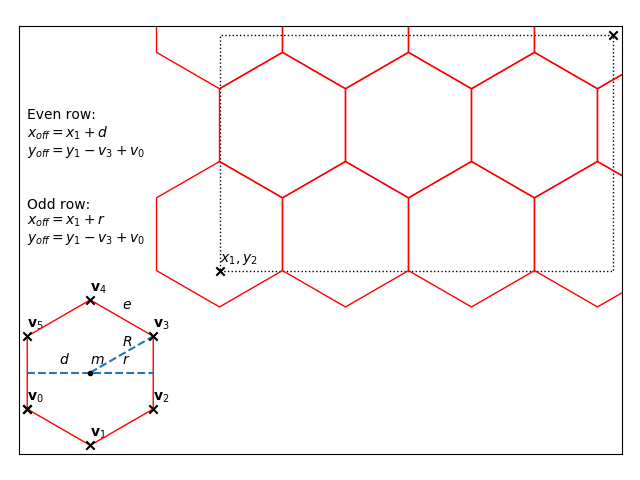
\includegraphics[scale=.7]{img/hexagons}
			\caption[Hexagon tessellation]{\textbf{Hexagon tessellation:} Located at the left bottom corner in red a hexagon defined by its geometric properties the 6 vertex vectors \{$\vec{v_0},...,\vec{v_5}$\} (black crosses), with center vector $\vec{m}$, edge length $e$, $R$ radius of the circumscribing circle, $r$ radius of the inscribed circle and $d$ the length of the short diagonal. Top right black dotted box are the bounds of an area which is tessellated by a hexagon grid in red. Each grid cell is translated from the origin hexagon at its position by computing the $x_{off}$ and $y_{off}$ offset with the presented equations at the left-hand side of the grid. }
			\label{fig:hexagon}
		\end{figure}
		% TODO DESCRIBE THE BINNING OF DATA AND WHAT WE WANT TO ACHIEVE
		Binning of raster data is easy we just have a point in polygon problem each points/pixels falling in hexagon are counted and aggregated through a function. In case of drivers of deforestation we count all driver classes per hexagon and compute ratios next we compute the sha \note{describe for each map how you build it}
		% TODO DESCRIBE CLIPPING
		As mentioned before for the visualization of the drivers of deforestation map we want to segment the hexagons with horizontal lines and each segment should represent the share of the direct deforestation driver within the tessellated area. To compute the split line for a certain hexagon we need the hexagon R computeable from the area of the hexagon equation \ref{eq:radius} and the rectangular bounds of the hexagon. We compute the relative share of an deforestation driver per hexagon this relative share can be used to compute the y-axis coordinate of an split line equation \ref{eq:percentage}. A regular hexagon can not only be presented in it vertex form as shown above. We can also use functions to define the hexagon shape. A hexagon consist of 2 picewise functions where each function consist of 3 linear functions restricted to an intervall. If we invert these functions we can use these functions to compute the x-coordinate of the split line with the previous computed y-coordinate Equations \ref{eq:left} and \ref{eq:right}. As a results we receive the solution matrix L which represents the horizontal line segment splitting the hexagon at the point where we want (driver ratio share) equation \ref{eq:line}. The solution matrix can be plugged in to a polygon split function which separates the hexagon polygon in a upper and lower part to do so we iterate over the hexagon vertices and decide if they are above or under the split line and append to a lower upper polygon. These list are our results \note{explain better split function}.
		\begin{equation}
		\label{eq:radius}
			R = \frac{\sqrt{2A}}{\sqrt[4]{27}}
		\end{equation}
		\begin{equation}
		\label{eq:percentage}
			y = \frac{P(y_2-y_1)}{100} + y_1
		\end{equation}
		\begin{equation}
		\label{eq:left}
			f^{-1}(y) =
			\begin{cases} 
				-\frac{y - y_1}{\tan{(\frac{\pi}{6}})} + \frac{x_1 + x_2}{2} & \text{if } y_1 \le y < y_1 + R\sin{(\frac{5\pi}{6})} \\
				x_1 & \text{if } y_1 + R\sin{(\frac{5\pi}{6})} \le y < R(\sin{(\frac{5\pi}{6})} + 1) \\
				\frac{y - y_2}{\tan{(\frac{\pi}{6}})} + \frac{x_1 + x_2}{2} & \text{if } R(\sin{(\frac{5\pi}{6})} + 1) \le y \le y_2
			\end{cases}
		\end{equation}
		\begin{equation}
		\label{eq:right}
			g^{-1}(y) = 
			\begin{cases} 
				\frac{y - y_1}{\tan{(\frac{\pi}{6}})} + \frac{x_1 + x_2}{2} & \text{if } y_1 \le y < y_1 + R\sin{(\frac{5\pi}{6})} \\
				x_2 & \text{if } y_1 + R\sin{(\frac{5\pi}{6})} \le y < R(\sin{(\frac{5\pi}{6})} + 1) \\
				-\frac{y - y_2}{\tan{(\frac{\pi}{6}})} + \frac{x_1 + x_2}{2} & \text{if } R(\sin{(\frac{5\pi}{6})} + 1) \le y \le y_2
			\end{cases}
		\end{equation}
		\begin{equation}
		\label{eq:line}
			\mathbf{L} =
			\begin{bmatrix}
				f^{-1}(y) & g^{-1}(y) \\
				y & y
			\end{bmatrix}
		\end{equation}
